\documentclass[tikz,border=10pt]{standalone}
\usepackage{amsmath,amssymb}
\usetikzlibrary{arrows.meta,calc,positioning}

\begin{document}
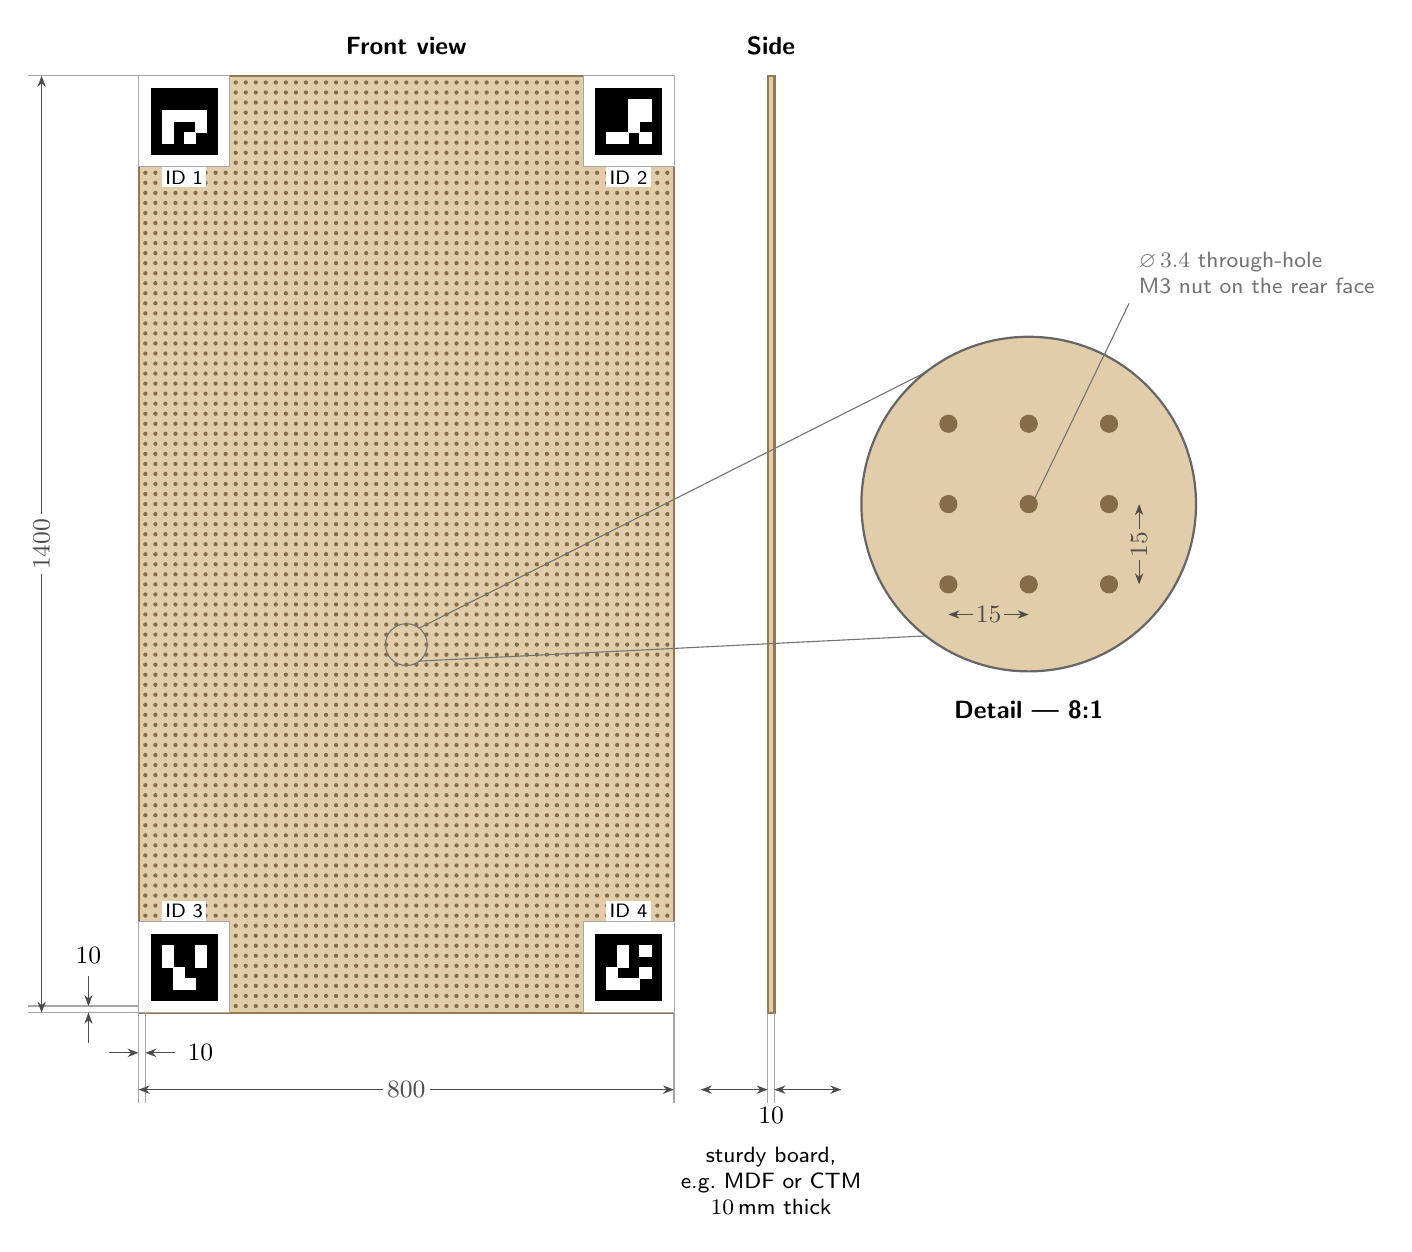
\begin{tikzpicture}[
    x=0.0085cm, y=0.0085cm,          % 1 drawing unit = 1 mm
    >={Stealth[length=4pt,width=3pt]},
    font=\sffamily\small,
    dim/.style={<->,thin,black!70},
    ext/.style={thin,black!35},
    lead/.style={thin,black!55},
  ]
  \definecolor{wood}{RGB}{226,205,171}
  \definecolor{woodE}{RGB}{150,120,80}

  %% ---------------- parameters (mm) ----------------
  \def\W{800}\def\H{1400}\def\P{15}\def\M{10}\def\T{10}

  %% ---------------- front view ----------------
  \fill[wood,draw=woodE,thick] (0,0) rectangle (\W,\H);
  \foreach \i in {0,...,52}{\foreach \j in {0,...,92}{
      \fill[woodE!90!black] ({\M+\i*\P},{\M+\j*\P}) circle (3.2);}}
  % ArUco markers: black code \AK + white border \AB (plate \AT x \AT mm),
  % outer corner of the border on the wall corner. Genuine DICT_4X4_50
  % patterns, generated by gen_aruco.py.
  % GEN ARUCO BEGIN
  \def\arucoA{1/3,2/3,3/3,4/3,1/2,4/2,1/1,3/1}% ID 1
  \def\arucoB{3/4,4/4,3/3,4/3,3/2,1/1,2/1,4/1}% ID 2
  \def\arucoC{1/4,4/4,1/3,4/3,2/2,2/1,3/1}% ID 3
  \def\arucoD{2/4,4/4,2/3,1/2,4/2,1/1,2/1,3/1}% ID 4
  \def\arucoE{2/4,3/4,4/4,1/3,4/3,1/2,2/2,1/1,2/1,4/1}% ID 5
  % GEN ARUCO END
  \def\AK{100}\def\AB{18}\pgfmathtruncatemacro{\AT}{\AK+2*\AB}
  \newcommand{\arucoF}[3]{% x0 y0 (lower-left of the plate), white-cell list
    \fill[white,draw=black!35,line width=0.3pt] (#1,#2) rectangle ++(\AT,\AT);
    \fill[black] ({#1+\AB},{#2+\AB}) rectangle ++(\AK,\AK);
    \foreach \c/\r in #3{
      \filldraw[white,line width=0.2pt] ({#1+\AB+\AK/6*\c},{#2+\AB+\AK/6*\r}) rectangle ++(\AK/6,\AK/6);}}
  \arucoF{0}{\H-\AT}{\arucoA}     \arucoF{\W-\AT}{\H-\AT}{\arucoB}
  \arucoF{0}{0}{\arucoC}          \arucoF{\W-\AT}{0}{\arucoD}
  \foreach \x/\y/\a/\t in {{\AT/2}/{\H-\AT}/north/1, {\W-\AT/2}/{\H-\AT}/north/2,
                           {\AT/2}/{\AT}/south/3,    {\W-\AT/2}/{\AT}/south/4}
    \node[anchor=\a,fill=white,inner sep=1.2pt,font=\sffamily\scriptsize] at (\x,\y) {ID \t};

  \node[above=1.5mm] at (\W/2,\H) {\bfseries Front view};

  %% ---------------- horizontal dimensions ----------------
  \foreach \x in {0,\M,\W}{\draw[ext] (\x,0) -- (\x,-135);}
  \draw[dim] (0,-115) -- node[fill=white,inner sep=1.5pt] {$800$} (\W,-115);
  \draw[dim,-{Stealth[length=4pt,width=3pt]}] (-45,-60) -- (0,-60);
  \draw[dim,-{Stealth[length=4pt,width=3pt]}] ({\M+45},-60) -- (\M,-60);
  \node[right=0.3mm] at ({\M+45},-60) {$10$};

  %% ---------------- vertical dimensions ----------------
  \foreach \y in {0,\M,\H}{\draw[ext] (0,\y) -- (-165,\y);}
  \draw[dim] (-145,0) -- node[fill=white,inner sep=1.5pt,rotate=90] {$1400$} (-145,\H);
  \draw[dim,-{Stealth[length=4pt,width=3pt]}] (-75,-45) -- (-75,0);
  \draw[dim,-{Stealth[length=4pt,width=3pt]}] (-75,{\M+45}) -- (-75,\M);
  \node[above=0.3mm] at (-75,{\M+45}) {$10$};

  %% ---------------- side view ----------------
  \def\SX{940}
  \fill[wood,draw=woodE,thick] (\SX,0) rectangle ({\SX+\T},\H);
  \node[above=1.5mm] at ({\SX+\T/2},\H) {\bfseries Side};
  \draw[ext] (\SX,0) -- (\SX,-135);
  \draw[ext] ({\SX+\T},0) -- ({\SX+\T},-135);
  \draw[dim] ({\SX-100},-115) -- (\SX,-115);
  \draw[dim] ({\SX+\T},-115) -- ({\SX+\T+100},-115);
  \node[below=1mm] at ({\SX+\T/2},-115) {$10$};
  \node[below=6mm,align=center,font=\sffamily\footnotesize] at ({\SX+\T/2},-115)
        {sturdy board,\\ e.g.\ MDF or CTM\\ $10$\,mm thick};

  %% ---------------- magnified detail ----------------
  \def\CX{1330}\def\CY{760}\def\CR{250}\def\K{8}
  \coordinate (src) at ({\M+26*\P},{\M+36*\P});
  \draw[lead] (src) circle ({\CR/\K});
  \draw[lead] ($(src)+(52:{\CR/\K})$) -- ($(\CX,\CY)+(128:\CR)$);
  \draw[lead] ($(src)+(-52:{\CR/\K})$) -- ($(\CX,\CY)+(232:\CR)$);

  \begin{scope}
    \clip (\CX,\CY) circle (\CR);
    \fill[wood] (\CX,\CY) circle ({\CR+5});
    \foreach \i in {-1,0,1}{\foreach \j in {-1,0,1}{
        \fill[woodE!90!black] ({\CX+\i*\P*\K},{\CY+\j*\P*\K}) circle ({1.7*\K});}}
    \draw[dim] ({\CX-\P*\K},{\CY-\P*\K-45}) -- ({\CX},{\CY-\P*\K-45})
          node[midway,fill=wood,inner sep=1pt]{$15$};
    \draw[dim] ({\CX+\P*\K+45},{\CY-\P*\K}) -- ({\CX+\P*\K+45},{\CY})
          node[midway,fill=wood,inner sep=1pt,rotate=90]{$15$};
  \end{scope}
  \draw[thick,black!60] (\CX,\CY) circle (\CR);
  \node[below=2.5mm,align=center] at (\CX,{\CY-\CR}) {\bfseries Detail --- 8:1};

  \draw[lead] ({\CX+0.7*1.7*\K},{\CY+0.7*1.7*\K}) -- ({\CX+150},{\CY+300})
        node[above right=0mm,align=left,font=\sffamily\footnotesize]
        {$\varnothing\,3.4$ through-hole\\ M3 nut on the rear face};
\end{tikzpicture}
\end{document}
